\documentclass[11pt,a4paper]{article}
\usepackage{iftex}
\ifPDFTeX
\usepackage[utf8]{inputenc}
\usepackage[T1]{fontenc}
\usepackage{lmodern}
\else
\usepackage{fontspec}
\setmainfont{lmroman10-regular.otf}[BoldFont=lmroman10-bold.otf,ItalicFont=lmroman10-italic.otf,BoldItalicFont=lmroman10-bolditalic.otf]
\setmonofont{lmmono10-regular.otf}
\fi
\usepackage[ngerman]{babel}
\usepackage[a4paper,margin=24mm]{geometry}
\usepackage{microtype}
\usepackage{amsmath,amssymb}
\usepackage{booktabs,longtable,tabularx,array}
\usepackage{enumitem}
\usepackage{xcolor}
\usepackage{graphicx}
\usepackage{caption}
\usepackage{xurl}
\usepackage{hyperref}

\definecolor{navy}{HTML}{12334A}
\definecolor{teal}{HTML}{146B75}
\definecolor{signal}{HTML}{A8391A}
\definecolor{gruen}{HTML}{1B6B4A}
\definecolor{softgrey}{HTML}{F1F3F5}
\hypersetup{colorlinks=true,linkcolor=navy,citecolor=teal,urlcolor=teal,
  pdftitle={Die Datenlücke schließen: geprüfte kostenlose Quellen für das S\&P-500-Ranking},
  pdfauthor={ETHack 2026}}
\urlstyle{same}

\newcolumntype{P}[1]{>{\raggedright\arraybackslash}p{#1}}
\newcommand{\tco}{\ensuremath{\mathrm{t\,CO}_{2}\mathrm{e}}}
\newcommand{\ja}{\textcolor{gruen}{\textbf{ja}}}
\newcommand{\nein}{\textcolor{signal}{\textbf{nein}}}

\setlength{\parindent}{0pt}
\setlength{\parskip}{5pt}
\setlength{\tabcolsep}{4pt}
\setlength{\emergencystretch}{2em}
\setlist{itemsep=3pt,topsep=4pt,leftmargin=*}
\renewcommand{\arraystretch}{1.17}
\setcounter{tocdepth}{2}
\captionsetup{font=small,labelfont=bf,labelsep=period,skip=6pt}

\newcommand{\befund}[1]{%
  \par\vspace{2pt}\noindent\colorbox{softgrey}{%
  \begin{minipage}{\dimexpr\linewidth-2\fboxsep}\small\vspace{3pt}#1\vspace{3pt}\end{minipage}}\par\vspace{4pt}}

\title{\textcolor{navy}{Die Datenlücke schließen}\\[4mm]
\large Was an kostenlosen Quellen wirklich zu holen ist --\\
jede einzeln am Endpunkt geprüft}
\author{ETHack 2026 -- Recherchebericht, Folgebericht zur Ranking-Auswertung}
\date{Alle Abrufe: 12.~September 2026}

\begin{document}
\maketitle

\begin{abstract}
\noindent
Der vorige Bericht hat zwei Lücken beziffert: die Emissionsreihe endet 2023, und nur 157 der 503 Indexmitglieder sind überhaupt bewertbar -- fast ausschließlich Schwerindustrie. Dieser Bericht durchsucht die freie Datenlandschaft nach Abhilfe und prüft jeden Kandidaten am echten Endpunkt statt in der Dokumentation. Ergebnis: \textbf{beide Lücken sind zu einem großen Teil schließbar.} Für die Zeit nach 2023 liefern zwei Wege Daten bis ins laufende Jahr~2026. Für die Abdeckung bringen zwei bisher übersehene Quellen zusammen 228 zusätzliche Firmen -- darunter eine, die im vorigen Bericht noch als \glqq nur mit Headless-Browser erreichbar\grqq{} eingeschätzt wurde und sich als direkter Excel-Download herausstellte. Außerdem fand sich eine maschinenlesbare Konzernstruktur aus SEC-Pflichtanlagen, die die handgepflegte Tochtertabelle ersetzt: 916\,290 Einträge für 478 der 500 Mütter. Vier geprüfte Kandidaten sind Sackgassen, und zwei brauchen einen kostenlosen Account. Vier zusätzlich angebundene Quellen -- Arbeitsunfälle, Giftstoffe, Regeltreue und ein physischer Nenner -- heben die Abdeckung auf 349 der 503 Firmen und liefern erstmals eine Achse, die nachweislich unabhängig von der CO$_2$-Intensitaet ist. Abschnitt~\ref{sec:reihenfolge} nennt die Umsetzungsreihenfolge, Abschnitt~\ref{sec:accounts} das, was du anlegen musst.
\end{abstract}

\vspace{2mm}
\befund{\textbf{Prüfmethode.} Kein Kandidat steht hier, weil er in einer Dokumentation erwähnt wird. Jeder wurde am 12.~September 2026 aufgerufen; bei jedem steht, was tatsächlich zurückkam -- einschließlich der Fälle, in denen das eine Fehlermeldung war.}

\tableofcontents
\newpage

\section{Ausgangslage}

Aus dem vorigen Bericht, zur Erinnerung:

\begin{itemize}
\item \textbf{Zeitliche Lücke.} Die EPA hat das Berichtsjahr 2024 trotz Meldefrist Mai~2025 bis heute nicht veröffentlicht. Ab Geschäftsjahr 2024 gibt es keine Emissionsdaten auf Firmenebene.
\item \textbf{Strukturelle Lücke.} 157 von 503 Firmen bewertbar. Versorger 90\,\%, Immobilien 10\,\%, Informationstechnologie 16\,\%. Die Rangliste misst faktisch, wer große Schornsteine betreibt.
\item \textbf{Achse B unvollständig.} Zwei von sechs Greenwashing-Warnsignalen berechenbar. Das stärkste -- die Lücke zwischen versprochenem und tatsächlichem Reduktionspfad -- fehlte mangels Zieldaten ganz.
\end{itemize}

\section{Die geprüfte Quellenlage}

\begin{table}[htbp]
\centering\small
\caption{Alle geprüften Kandidaten, Stand 12.09.2026}
\label{tab:quellen}
\begin{tabularx}{\textwidth}{P{3.0cm} P{3.5cm} P{1.5cm} P{1.8cm} X}
\toprule
\textbf{Quelle} & \textbf{Liefert} & \textbf{bis FJ} & \textbf{Zugang} & \textbf{Prüfergebnis} \\
\midrule
EPA CAMPD & Scope 1, Kraftwerke, CEMS-gemessen & \textbf{2026} & Schlüssel & läuft; \texttt{DEMO\_KEY} nur 10 Anfragen/Std. \\
PUDL auf Zenodo & EPA-CEMS-Spiegel 1995--2026 & \textbf{2026} & frei & Public Domain, 4{,}5~GB Stundenwerte \\
PUDL SEC-Ex-21 & Konzern-Tochter-Struktur & 2026 & frei & 916\,290 Einträge, 478 von 500 Müttern \\
SBTi-Excel & Zielstatus, Zwischenziele & \textbf{2026} & frei & direkter xlsx-Download, 15\,605 Organisationen \\
SEC-Volltextsuche & selbstberichtete Mengen & \textbf{2026} & frei & 215 Indexfirmen, Extraktion nötig \\
CARB SB 253 & Scope 1+2, verpflichtend & 2025 & frei & Portal offen seit 01.09., Frist 10.11.2026 \\
EIA API v2 & Brennstoff je Kraftwerk & 2026 & Schlüssel & Gegenprobe zu CEMS \\
\midrule
CDP offen & nur Städte und Regionen & 2025 & frei & \nein{} -- keine Firmendaten im offenen Portal \\
iShares/BlackRock & Fonds-Kennzahlen & 2026 & frei & \nein{} -- nur Fondsaggregate, keine Einzelwerte \\
TPI & Transitionsbewertung & 2026 & frei & \nein{} -- Lizenz untersagt automatisiertes Auslesen \\
Climate TRACE & Anlagen weltweit & 2024 & frei & \nein{} -- Feld \texttt{Owners} bleibt leer \\
\bottomrule
\end{tabularx}
\end{table}

\begin{figure}[htbp]
\centering
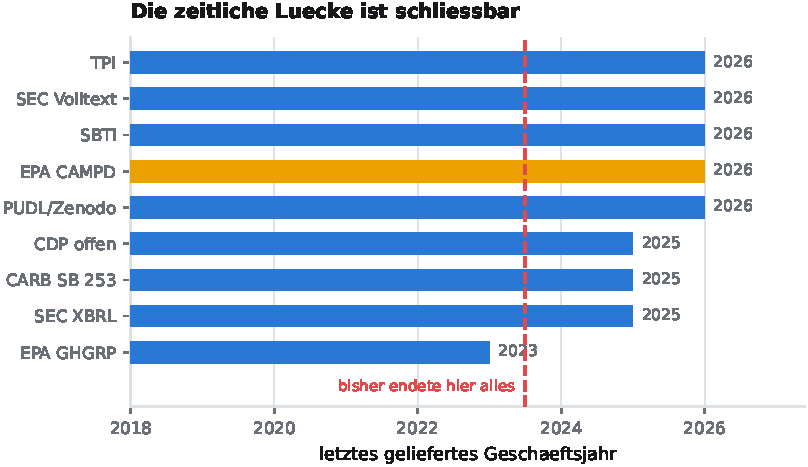
\includegraphics[width=0.9\textwidth]{figures/quellenlage.pdf}
\caption{Wie weit jede Quelle zeitlich reicht. Orange markiert die eine, die einen Schlüssel verlangt.}
\label{fig:quellenlage}
\end{figure}

\section{Lücke 1: die Zeit nach 2023}

\subsection{EPA CAMPD -- ein anderer Meldeweg für dieselben Kraftwerke}

Das Treibhausgas-Meldeprogramm (GHGRP) und die Clean Air Markets Program Data (CAMPD) stammen beide von der EPA, haben aber nichts miteinander zu tun. GHGRP ist eine jährliche Selbstmeldung mit langem Veröffentlichungsvorlauf. CAMPD kommt aus der kontinuierlichen Emissionsmessung am Schornstein, wird quartalsweise veröffentlicht und hat zwei bis drei Monate Verzug.

Der Abruf am 12.~September 2026 lieferte für die Jahre 2024, 2025 \emph{und} 2026 Datensätze -- rund 4\,000 Blockjahre je Jahr. Die zeitliche Lücke existiert für den Stromsektor schlicht nicht.

Zwei Eigenschaften machen CAMPD über die Aktualität hinaus wertvoll:

\begin{enumerate}
\item \textbf{Gemessen statt gerechnet.} CEMS misst am Schornstein. GHGRP-Werte werden überwiegend aus Brennstoffmengen hochgerechnet.
\item \textbf{Eigentümer und Betreiber getrennt.} Das Feld \texttt{ownerOperator} sieht so aus:
\begin{quote}\footnotesize\ttfamily
Alabama Power Company (Owner)|Alabama Power Company (Operator)
\end{quote}
Damit lässt sich die Zurechnung nach Equity Share \emph{und} nach operativer Kontrolle rechnen. Das war Schwachstelle~9 des vorigen Berichts: eine Ermessensentscheidung, die unsichtbar im Code steckte. Sie wird jetzt zu einer weiteren Dimension der Unsicherheitsanalyse.
\end{enumerate}

\befund{\textbf{Einschränkung, und zwar eine harte.} CAMPD deckt nur Anlagen der Emissionshandelsprogramme ab -- praktisch also Stromerzeugung. Raffinerien, Zementwerke, Stahl und Chemie erscheinen nicht. Für diese Branchen bleibt es bei 2023, bis die EPA das Berichtsjahr 2024 veröffentlicht.}

\subsection{PUDL -- derselbe Datensatz ohne Schlüssel}

Die Catalyst Cooperative veröffentlicht unter dem Namen PUDL aufbereitete US-Energiedaten auf Zenodo. Der Datensatz \emph{PUDL Raw EPA Hourly CEMS} (zuletzt 6.~September 2026) enthält die Stundenwerte von 1995 bis 2026, als Public Domain, ohne Anmeldung. 4{,}5~GB für die Stundenreihe, dazu kleinere Tabellen mit den Zuordnungen zwischen EPA- und EIA-Kennungen sowie Eigentumsanteilen aus dem EIA-Formular 860.

Damit gibt es für dieselbe Datengrundlage zwei Wege: den bequemen über die API mit Schlüssel und den schlüsselfreien über Zenodo mit mehr Rechenarbeit. Für einen Hackathon ist der erste richtig, für einen unbeaufsichtigt laufenden Dienst der zweite.

\section{Lücke 2: die Abdeckung}

\subsection{SBTi -- die Fehleinschätzung aus dem vorigen Bericht}

Im vorigen Bericht stand, die Science Based Targets initiative habe kein öffentliches API, man müsse die Dashboard-Seite mit einem Headless-Browser abgreifen, Aufwand zwei bis drei Stunden. Das war falsch. Der Pfad \texttt{/download/excel} leitet auf eine veröffentlichte Tabelle weiter und liefert den vollständigen Datensatz:

\begin{quote}\footnotesize\ttfamily
https://sciencebasedtargets.org/download/excel \\
$\rightarrow$ 302 $\rightarrow$ xlsx, 2{,}3~MB, 15\,605 Zeilen, 22 Spalten
\end{quote}

Enthalten sind \texttt{company\_name}, \texttt{isin}, \texttt{lei}, Sektor, und je Organisation der Status von Nahziel, Langfristziel und Netto-null-Ziel samt Zieljahren und Klassifizierung (1{,}5~Grad, deutlich unter 2~Grad, 2~Grad).

\begin{table}[htbp]
\centering\small
\caption{Was der SBTi-Datensatz für den S\&P 500 hergibt (Abgleich über normalisierte Firmennamen)}
\label{tab:sbti}
\begin{tabular}{lr}
\toprule
Indexfirmen mit SBTi-Eintrag & 241 von 503 (48\,\%) \\
davon mit geprüftem Nahziel & 209 \\
davon mit ausgewiesenem Zwischenzieljahr & 209 \\
davon mit zurückgezogener Zusage & \textbf{50} \\
Firmen, die heute \emph{keine} Emissionsdaten haben & \textbf{173} \\
\bottomrule
\end{tabular}
\end{table}

Damit werden drei der sechs Greenwashing-Warnsignale berechenbar, die bisher fehlten: das Vorhandensein von Zwischenzielen, die wissenschaftliche Prüfung des Ziels, und -- neu und im vorigen Bericht gar nicht vorgesehen -- der Rückzug einer einmal gegebenen Zusage.

\befund{\textbf{Das interessanteste Feld im ganzen Datensatz} ist \texttt{Commitment removed}. 50 Indexfirmen haben sich ein Klimaziel gesetzt und es später zurückgezogen. Das ist kein Indiz, das man aus Textanalyse ableiten müsste, sondern eine protokollierte Tatsache mit Datum. Als Glaubwürdigkeitssignal ist es schwer wegzudiskutieren.}

\subsection{SEC-Volltextsuche -- Selbstauskunft aus Pflichtberichten}

Die Volltextsuche der SEC (\texttt{efts.sec.gov}) ist ohne Anmeldung abrufbar und liefert strukturiertes JSON mit CIK je Treffer. Eine Suche nach \texttt{"Scope 1"} in 10-K-Berichten seit Januar~2025 ergibt 787 Dokumente, davon 131 von Indexmitgliedern. Über drei Suchbegriffe zusammengenommen: 215 Indexfirmen, davon 124 ohne heutige Emissionsdaten.

Entscheidend ist aber nicht, wie viele Firmen das Wort nennen, sondern bei wie vielen sich eine Zahl herausziehen lässt. Eine erste Stichprobe mit einem naiven Muster fand nur bei einer von sechs Firmen etwas -- die meisten Nennungen stehen in Risikohinweisen (\glqq Vorschriften könnten uns verpflichten, Scope-1-Emissionen zu melden\grqq), nicht in Offenlegungen. Mit drei verbesserten Mustern stieg die Ausbeute an einer Stichprobe von 40 Firmen auf \textbf{80\,\%}.

\befund{\textbf{Was diese 80\,\% sind und was nicht.} Gemessen wurde, ob in der Nähe von \glqq Scope 1\grqq{} eine Zahl mit Mengeneinheit steht. Ob diese Zahl die gesuchte Gesamtmenge ist -- und nicht ein Zieljahr, ein Prozentsatz oder der Scope-2-Wert --, ist damit \emph{nicht} geprüft. Die Trefferquote ist eine Obergrenze für die Ausbeute und sagt nichts über die Genauigkeit. Vor dem Produktiveinsatz braucht es eine Stichprobe von etwa 20 handgeprüften Firmen.}

\subsection{Konzernstrukturen aus SEC-Pflichtanlagen}

Die im vorigen Bericht am meisten kritisierte Stelle war die handgepflegte Tochter-Konzern-Tabelle mit rund 280 Einträgen: \glqq Handarbeit und damit die am wenigsten skalierbare Stelle der ganzen Pipeline\grqq.

Jedes 10-K enthält als Anlage~21 die Liste der Tochtergesellschaften. PUDL hat diese Anlagen für alle Einreichungen ausgewertet und als Tabelle veröffentlicht:

\begin{table}[htbp]
\centering\small
\caption{\texttt{core\_sec10k\_\_quarterly\_exhibit\_21\_company\_ownership}, gefiltert auf S\&P-500-Mütter}
\label{tab:ex21}
\begin{tabular}{lr}
\toprule
Tochtereinträge insgesamt & 3\,800\,706 \\
davon unter S\&P-500-Müttern & 916\,290 \\
abgedeckte Mütter & \textbf{478 von 500} \\
Einträge mit Beteiligungsquote & 99\,117 \\
\bottomrule
\end{tabular}
\end{table}

Die Stichprobe bestätigt die Qualität: Southern Company führt 240 Töchter, darunter Alabama Power und Georgia Power; NextEra führt Florida Power \& Light; Berkshire Hathaway führt MidAmerican Energy und Kern River Gas Transmission. Das sind genau die Zuordnungen, die bisher von Hand eingetragen wurden -- hier stehen sie aus der Pflichtanlage einer Börsenaufsicht.

\section{Was bald von selbst kommt}

Kalifornien hat mit SB~253 eine Offenlegungspflicht beschlossen, die jede Firma mit mehr als einer Milliarde Dollar Umsatz und Geschäft in Kalifornien betrifft -- praktisch also den gesamten S\&P~500. Der Stand:

\begin{itemize}
\item Die Durchführungsverordnung wurde am 26.~Februar 2026 von der kalifornischen Umweltbehörde beschlossen.
\item Die ursprüngliche Frist zum 10.~August 2026 wurde am 24.~Juni auf den \textbf{10.~November 2026} verschoben.
\item Seit dem 1.~September 2026 ist eine Einreichungsplattform offen.
\item Die eingereichten Berichte werden über ein öffentliches Register zugänglich gemacht.
\item Scope~1 und~2 ab 2026, \textbf{Scope~3 ab 2027}.
\end{itemize}

\befund{\textbf{Das ist die strukturelle Lösung, nicht nur ein Notbehelf.} Wenn diese Pflicht greift, existiert erstmals eine geprüfte, verpflichtende und kostenlose Scope-1-und-2-Quelle für nahezu den gesamten Index -- und ab 2027 auch für Scope~3, also für genau den Teil, den heute keine freie Quelle abdeckt. Für dieses Hackathon-Wochenende kommt sie zwei Monate zu spät. Für die Architektur heißt das: einen \texttt{CarbSb253Source}-Platzhalter vorsehen, damit die Umstellung später ein Connector und keine Neuentwicklung ist.}

\section{Was sich als Sackgasse erwies}

Diese vier wurden geprüft und bringen nichts -- das gehört genauso dokumentiert wie die Treffer.

\paragraph{CDP.} Es gibt tatsächlich ein offenes Datenportal unter \texttt{data.cdp.net}, und es antwortet. Es enthält 40 Datensätze -- alle über Städte, Bundesstaaten und Regionen. \emph{Firmendaten sind nicht darunter.} Die Aussage des Ausgangspapiers, der beste Datensatz liege hinter einer Bezahlschranke, bestätigt sich; der offene Teil betrifft ein anderes Messobjekt.

\paragraph{BlackRock und iShares.} Die Fondsseiten veröffentlichen Bestandslisten und Nachhaltigkeitskennzahlen. Die Kennzahlen sind jedoch \emph{Fondsaggregate} -- eine gewichtete durchschnittliche Kohlenstoffintensität für den ganzen Fonds, geliefert von MSCI. Einzelwerte je Unternehmen stehen nicht darin. Für eine Rangliste der Einzelfirmen ist das wertlos; für eine spätere Portfolio-Gegenprobe ist es als Vergleichszahl brauchbar.

\paragraph{Transition Pathway Initiative.} Fachlich die beste freie Bewertung, die gefunden wurde, und sie deckt auch Banken und Immobilien ab. Aber die Nutzungsbedingungen der LSE sind eindeutig: Der Einsatz \glqq automatisierter Werkzeuge (einschließlich Bots, Scraper oder Spider), um die Daten abzurufen, zu extrahieren oder zu indizieren\grqq{} ist genehmigungspflichtig. Ebenso die \glqq Erstellung eines Index oder Fonds\grqq{} auf Basis dieser Daten -- also genau die Bonusaufgabe der Challenge. Manuelle Einsicht zur Validierung ist erlaubt, eine Einbindung in die Pipeline nicht.

\paragraph{Climate TRACE.} Wie im vorigen Bericht: Die API läuft, aber das Feld \texttt{Owners} kommt leer zurück. Ohne Eigentümerzuordnung sind Anlagendaten für ein Firmenranking nicht verwendbar.

\section{Was das zusammen bedeutet}

\begin{figure}[htbp]
\centering
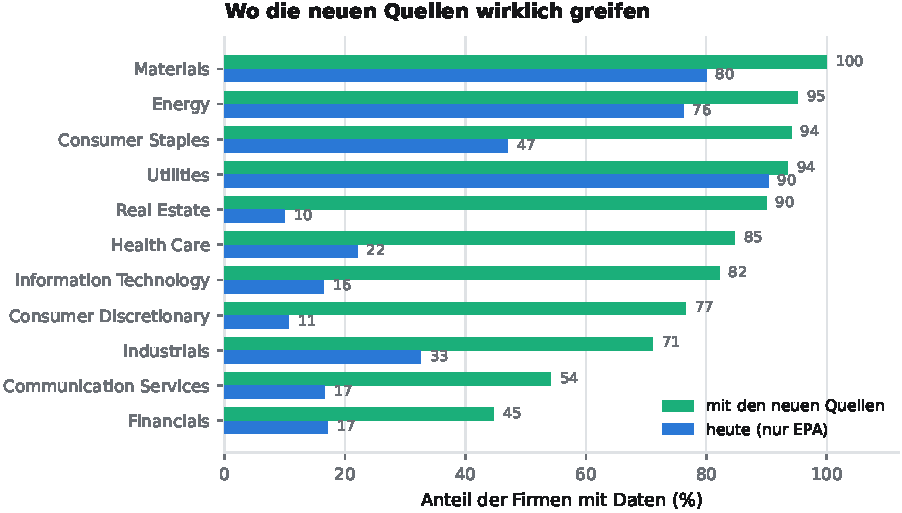
\includegraphics[width=0.92\textwidth]{figures/abdeckung_vorher_nachher.pdf}
\caption{Abdeckung je GICS-Sektor, heute gegen erreichbar mit den neuen Quellen.}
\label{fig:vorhernachher}
\end{figure}

\begin{figure}[htbp]
\centering
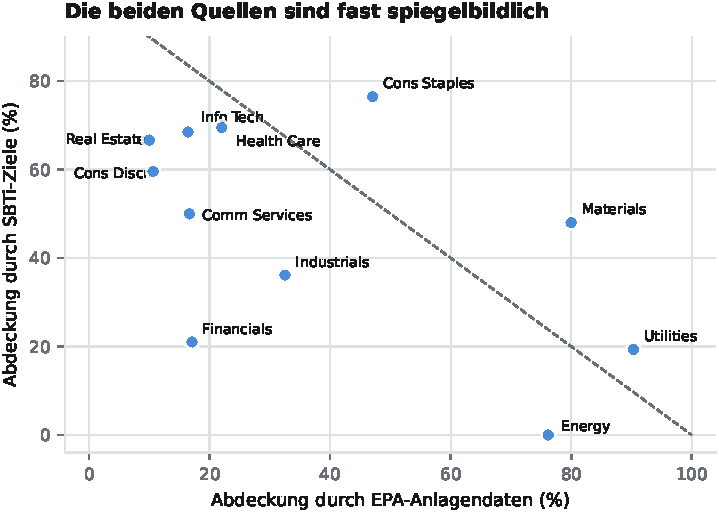
\includegraphics[width=0.88\textwidth]{figures/komplementaritaet.pdf}
\caption{EPA-Anlagendaten und SBTi-Ziele decken gegenläufige Hälften des Index ab. Die gestrichelte Linie markiert, wo sich beide Anteile zu 100 ergänzen würden.}
\label{fig:komplement}
\end{figure}

Die Komplementarität in Abbildung~\ref{fig:komplement} ist kein Zufall. Die EPA erfasst, wer Schornsteine betreibt. Die SBTi erfasst, wer sich freiwillig ein Ziel gesetzt hat -- und das tun bevorzugt Firmen mit geringem physischem Fußabdruck und hoher Markenempfindlichkeit. Energie: 0\,\% SBTi-Abdeckung bei 76\,\% EPA-Abdeckung. Informationstechnologie: 68\,\% SBTi bei 16\,\% EPA.

\subsection{Die ehrliche Bilanz}

\begin{figure}[htbp]
\centering
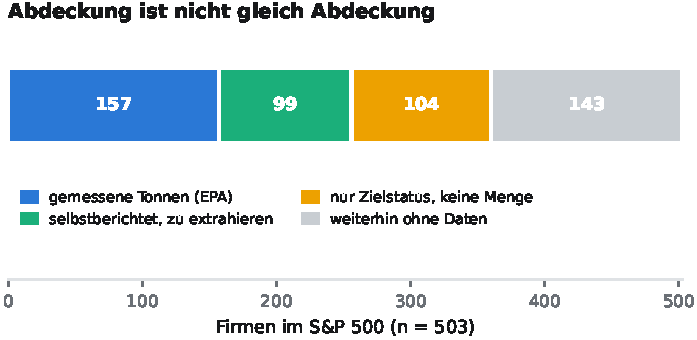
\includegraphics[width=0.92\textwidth]{figures/datenart.pdf}
\caption{Die 503 Indexmitglieder nach Art der verfügbaren Daten.}
\label{fig:datenart}
\end{figure}

Eine Gesamtzahl von \glqq 385 Firmen mit mindestens einer Quelle\grqq{} wäre genau die aufgeblasene Kennzahl, die der vorige Bericht kritisiert hat. Die Quellen liefern nicht dasselbe:

\begin{table}[htbp]
\centering\small
\caption{Abdeckung nach Art der Daten}
\label{tab:bilanz}
\begin{tabular}{lrl}
\toprule
\textbf{Art} & \textbf{Firmen} & \textbf{Herkunft} \\
\midrule
gemessene Tonnen & 157 & EPA-Anlagendaten, wie bisher \\
selbstberichtete Tonnen, noch zu extrahieren & 99 & SEC-Volltext, 80\,\% Ausbeute angesetzt \\
nur Zielstatus, keine Menge & 104 & SBTi ohne Emissionsquelle \\
weiterhin ohne Daten & 143 & -- \\
\midrule
\textbf{mit einer Emissionsmenge} & \textbf{256} & 51\,\% des Index \\
\textbf{mit irgendeiner Information} & \textbf{385} & 77\,\% des Index \\
\bottomrule
\end{tabular}
\end{table}

\befund{\textbf{Die belastbare Zahl ist 256, nicht 385.} Eine Kernnote braucht eine Menge. SBTi liefert keine -- der Zielstatus gehört auf Achse~B und darf die Abdeckung der Kernnote nicht schönrechnen. Und die 99 selbstberichteten sind eine Erwartung auf Basis einer Stichprobe von 40 Firmen, keine gezählten Werte. Belastbar ist heute: 157 gemessen, ein plausibler Aufwuchs auf rund 256, und 143 Firmen, für die es weiterhin nichts gibt.}

\section{Umsetzungsreihenfolge}
\label{sec:reihenfolge}

Sortiert nach Wirkung je Aufwand. Die ersten drei sind für ein Hackathon-Wochenende realistisch.

\paragraph{S1 -- SBTi einbinden (Aufwand: erledigt).}
Der Connector ist geschrieben und der Datensatz liegt im Cache. Es fehlt der Abgleich über ISIN statt über Firmennamen, was die heutigen 48\,\% Trefferquote noch anheben dürfte. Bringt: drei Greenwashing-Signale und 173 Firmen auf Achse~B. \emph{Höchste Wirkung, geringster Restaufwand.}

\paragraph{S2 -- CAMPD für Periode B (Aufwand: zwei Stunden nach Schlüsselerhalt).}
Connector ist geschrieben. Sobald der Schlüssel da ist: Daten für 2024 bis 2026 ziehen, über \texttt{ownerOperator} zuordnen, und den Stromsektor damit bis ins laufende Jahr fortschreiben. Für alle anderen Branchen bleibt die Kennzeichnung \glqq Stand 2023\grqq. Das ist ein ehrlicheres Ergebnis als eine einheitliche Fortschreibung.

\paragraph{S3 -- Tochtertabelle durch Exhibit 21 ersetzen (Aufwand: ein halber Tag).}
Die 916\,290 Einträge über die Mutter-CIK anbinden, gegen die heutige Handtabelle validieren, Abweichungen prüfen. Beseitigt die am wenigsten skalierbare Stelle der Pipeline und dürfte die Zuordnungsquote über die heutigen 48\,\% der Emissionen heben.

\paragraph{S4 -- Equity Share gegen operative Kontrolle (Aufwand: eine Stunde).}
Mit dem getrennten Eigentümer- und Betreiberfeld beide Zurechnungsregeln rechnen und als weitere Dimension in die Unsicherheitsanalyse geben. Schließt Schwachstelle~9 des vorigen Berichts.

\paragraph{S5 -- SEC-Volltextextraktion (Aufwand: ein bis zwei Tage).}
Die aufwendigste Position, und die einzige, die die Abdeckung wirklich erhöht. Reihenfolge: Muster verfeinern, an 20 handgeprüften Firmen die Genauigkeit messen, erst dann in die Pipeline aufnehmen -- und jeden extrahierten Wert als \glqq selbstberichtet, unbestätigt\grqq{} kennzeichnen, getrennt von den gemessenen EPA-Werten.

\paragraph{S6 -- Platzhalter für SB 253 (Aufwand: eine Stunde).}
Einen \texttt{CarbSb253Source} anlegen, der heute nichts liefert, und die Feldnamen nach dem CARB-Meldeschema benennen. Wenn im November die Berichte kommen, ist das ein Connector und keine Neuentwicklung.

\paragraph{S7 -- EIA als Gegenprobe (Aufwand: ein halber Tag).}
Aus den Brennstoffmengen des EIA-Formulars 923 lassen sich Emissionen mit Standardfaktoren nachrechnen. Wo CEMS und EIA weit auseinanderliegen, stimmt etwas nicht. Das ist die einzige verfügbare unabhängige Kontrolle der Zurechnung -- und damit wertvoller, als es nach Fleißarbeit aussieht.

\section{Was du anlegen musst}
\label{sec:accounts}

\begin{table}[htbp]
\centering\small
\caption{Benötigte Zugänge -- beide kostenlos und sofort}
\label{tab:accounts}
\begin{tabularx}{\textwidth}{P{3.2cm} P{5.4cm} X}
\toprule
\textbf{Dienst} & \textbf{Registrierung} & \textbf{Wofür} \\
\midrule
EPA CAM API & \url{https://www.epa.gov/power-sector/cam-api-portal} & \textbf{Wichtigster Punkt.} Schließt die Periode-B-Lücke für den Stromsektor. Ohne Schlüssel greift \texttt{DEMO\_KEY} mit 10 Anfragen je Stunde -- für einen Testlauf genug, für den Betrieb nicht. \\
EIA Open Data & \url{https://www.eia.gov/opendata/register.php} & Gegenprobe über Brennstoffmengen (S7). Nachrangig. \\
\bottomrule
\end{tabularx}
\end{table}

Den Schlüssel setzt du als Umgebungsvariable, der Connector liest sie selbst:

\begin{quote}\footnotesize\ttfamily
export EPA\_CAMD\_API\_KEY="..." \\
.venv/bin/python scripts/01\_fetch.py campd\_emission campd\_facility
\end{quote}

Alles andere in diesem Bericht läuft ohne Anmeldung. Kaggle wird nicht mehr gebraucht -- der dort kursierende ESG-Snapshot war ohnehin nur Vergleichsmaßstab und ist durch SBTi als Achse-B-Quelle abgelöst.

\section{Vier weitere Dimensionen -- und was sie wirklich beitragen}

Schwachstelle~4 des vorigen Berichts lautete: drei Kennzahlen sind zu wenig, und zwei davon messen fast dasselbe. Die Folge war messbar -- die geometrische Aggregation, methodisch das Herzstück, veränderte im Median nichts, weil es bei korrelierten Kennzahlen nichts zu kompensieren gibt. Vier weitere Quellen wurden daraufhin angebunden und an genau dieser Frage gemessen: Erreichen sie genug Firmen, und sind sie tatsächlich unabhängig?

\begin{figure}[htbp]
\centering
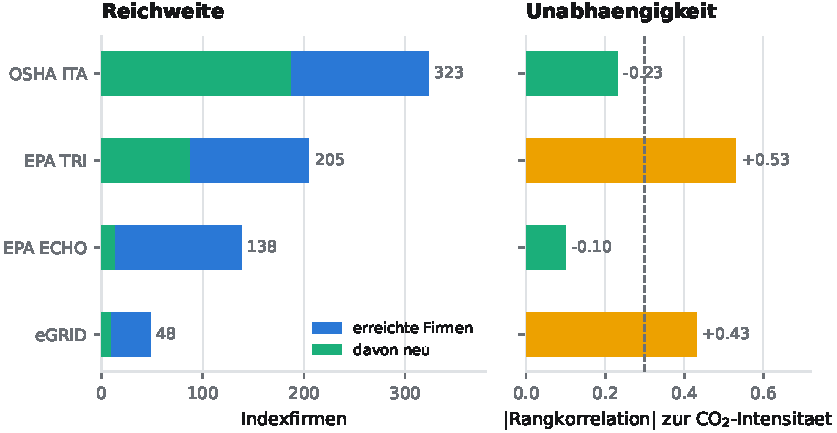
\includegraphics[width=0.97\textwidth]{figures/neue_dimensionen.pdf}
\caption{Links die Zahl erreichter Indexfirmen, grün der Teil ohne bisherige Emissionsdaten. Rechts der Betrag der Rangkorrelation zur CO\textsubscript{2}-Intensität; unter 0{,}3 (gestrichelt) trägt eine Kennzahl eigenständige Information.}
\label{fig:dimensionen}
\end{figure}

\begin{table}[htbp]
\centering\small
\caption{Die vier Dimensionen, gemessen statt geschätzt}
\label{tab:dimensionen}
\begin{tabularx}{\textwidth}{P{2.5cm} P{3.3cm} r r r X}
\toprule
\textbf{Quelle} & \textbf{Dimension} & \textbf{Firmen} & \textbf{neu} & \textbf{$\rho$} & \textbf{Urteil} \\
\midrule
OSHA ITA & Arbeitssicherheit (DART) & \textbf{323} & 187 & $-0{,}23$ & breiteste Abdeckung aller geprüften Quellen, weitgehend unabhängig \\
EPA TRI & Giftstofffreisetzung & 205 & 87 & $+0{,}53$ & teilredundant zu CO\textsubscript{2}; eigenständig ist das Krebserreger-Kennzeichen \\
EPA ECHO & Regeltreue & 138 & 13 & $-0{,}10$ & \textbf{die gesuchte unabhängige Achse} \\
eGRID & t CO\textsubscript{2} je MWh & 48 & 9 & $+0{,}43$ & richtiger Nenner, aber nur für Stromerzeuger \\
\bottomrule
\end{tabularx}
\end{table}

\subsection{Der physische Nenner}

Jede Intensität hing bisher am Umsatz. Das hat einen Konstruktionsfehler: Der Nenner reagiert auf den Strompreis. Ein Versorger sieht in einem Jahr mit hohen Großhandelspreisen sauberer aus, ohne eine Tonne weniger auszustoßen.

Für Stromerzeuger löst die eGRID-Datenbank der EPA das, ohne dass etwas gerechnet werden muss: Sie führt Emissionen und Erzeugung auf Kraftwerksebene bereits zusammen, einschließlich Betreiber- und Versorgernamen. 48 Indexfirmen bekommen daraus eine Kennzahl in \tco{} je Megawattstunde, davon 24 Versorger; abgedeckt sind 1{,}77 der 2{,}64 Milliarden fossil erzeugten Megawattstunden.

Die Rangkorrelation zur umsatzbasierten Intensität beträgt $\rho = 0{,}43$ ($n = 39$, $p = 0{,}007$) -- verwandt, aber deutlich nicht dasselbe. Der Wechsel des Nenners verschiebt die Rangfolge also spürbar.

\befund{\textbf{Und eine Warnung dazu.} Die Kennzahl ist nur für Firmen aussagekräftig, deren Geschäft die Stromerzeugung ist. Im Datensatz erscheinen auch Walmart mit sieben Anlagen und GE Aerospace mit einer einzigen, die auf 4{,}4~\tco{} je MWh kommt -- ein Wert, der nichts über den Konzern aussagt, sondern über ein Blockheizkraftwerk. Angewendet gehört die Kennzahl auf die 24 Versorger, nicht auf alle 48 Treffer. Das ist genau der Grundsatz, nur branchenrelevante Größen zu messen.}

\subsection{Die Achse, die bisher fehlte}

ECHO führt je Anlage die dokumentierte Konformität mit Umweltauflagen: Strafen, Inspektionen und eine Zeichenkette mit einem Zeichen je Quartal über drei Jahre. Für die Zuordnung gibt es hier einen Weg, der ohne Namensabgleich auskommt: Sowohl die GHGRP-Anlagen als auch ECHO tragen dieselbe FRS-Kennung. \textbf{13\,370 ECHO-Anlagen ließen sich so verlustfrei an bereits zugeordnete Konzerne hängen} -- die präziseste Verknüpfung, die dieses Projekt bisher hat.

Entscheidend ist das Ergebnis der Unabhängigkeitsprüfung: $\rho = -0{,}10$ zur CO\textsubscript{2}-Intensität, bei $n = 118$ und $p = 0{,}295$ also kein nachweisbarer Zusammenhang. Regeltreue und Emissionsintensität messen verschiedene Dinge.

\befund{\textbf{Warum das die wichtigste der vier ist.} Die multiplikative Aggregation war bisher wirkungslos, weil alle Kennzahlen in dieselbe Richtung zeigten. Mit einer unkorrelierten Achse bekommt sie erstmals etwas zu tun: Eine Firma mit guter CO\textsubscript{2}-Bilanz und schlechter Regeltreue kann das eine nicht mehr mit dem anderen zurückkaufen. Governance ist zudem der Teilbereich, bei dem kommerzielle Anbieter am stärksten auseinanderliegen -- hier wird sie aus dokumentiertem Verhalten gebildet statt aus Richtlinientexten.}

\subsection{Arbeitssicherheit -- die größte Reichweite}

Die OSHA-Meldungen nach Formular 300A liefern 1\,176\,137 Betriebsstätten-Jahre für 2023 bis 2025, daraus die DART-Rate: Fälle mit Arbeitsausfall oder Einschränkung je 100 Vollzeitkräfte. Mit \textbf{323 erreichten Indexfirmen ist das die breiteste aller geprüften Quellen} -- 187 davon haben keine Emissionsdaten. Die Korrelation zur CO\textsubscript{2}-Intensität liegt bei $\rho = -0{,}23$.

Die Spitzenwerte sind plausibel und zeigen zugleich, dass die Kennzahl Branchenstruktur misst: Southwest Airlines 11{,}3, FedEx 10{,}7 über 1566 Betriebsstätten, UPS 6{,}5 über 1477. Logistik und Luftfahrt sind körperlich fordernd. Auch diese Kennzahl gehört deshalb branchenrelativ normalisiert, nicht absolut verglichen.

\subsection{Giftstoffe -- nützlich, aber nicht unabhängig}

TRI erreicht 205 Indexfirmen, 87 davon neu, und bringt einen Vorteil mit, den keine andere Quelle hat: Die EPA führt im Feld \texttt{standard\_parent\_co\_name} bereits einen bereinigten Konzernnamen -- die Zuordnungsarbeit ist geleistet. Insgesamt 286 Millionen Pfund Freisetzung, davon 26{,}4 Millionen Pfund krebserregender Stoffe.

Die Unabhängigkeitsprüfung fällt allerdings gemischt aus: $\rho = +0{,}53$ zur CO\textsubscript{2}-Intensität ($n = 109$, $p < 0{,}001$). Anlagen, die viel CO\textsubscript{2} ausstoßen, setzen auch viel anderes frei. Als eigene Achse taugt die Gesamtmenge damit nur begrenzt. Eigenständig ist dagegen der \emph{Anteil krebserregender Stoffe} an der Freisetzung -- eine Gewichtung, die die reine Massensumme nicht hergibt.

\subsection{Was das für die Abdeckung heißt}

\begin{figure}[htbp]
\centering
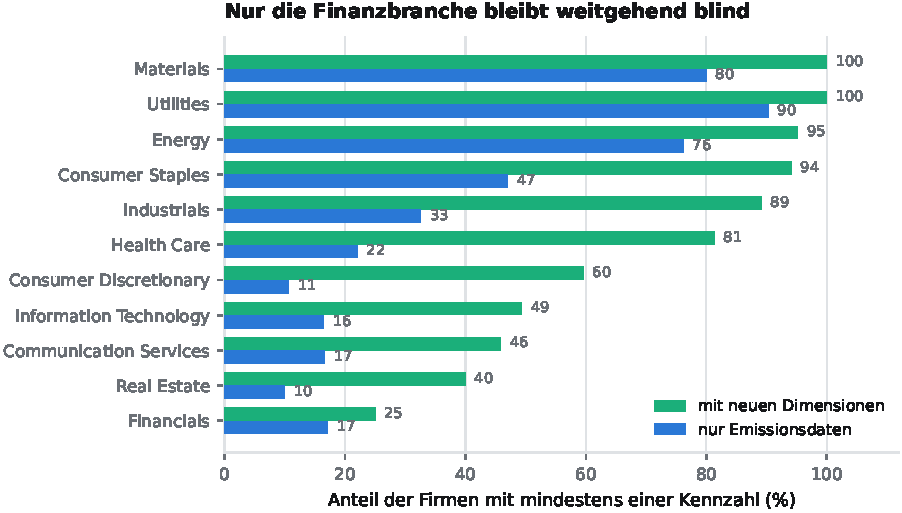
\includegraphics[width=0.92\textwidth]{figures/dimension_abdeckung.pdf}
\caption{Anteil der Firmen je Sektor mit mindestens einer Kennzahl, vorher und nachher.}
\label{fig:dimabdeckung}
\end{figure}

339 Indexfirmen erhalten mindestens eine der vier Dimensionen, 192 davon hatten bisher keine Emissionsdaten. Zusammen mit den gemessenen Emissionen sind das \textbf{349 von 503 Firmen}, also 69 Prozent. Versorger und Grundstoffe erreichen 100 Prozent, Industrie springt von 33 auf 89, Gesundheit von 22 auf 81.

\befund{\textbf{Die Finanzbranche bleibt das ungelöste Problem.} 19 von 76 Firmen, also 25 Prozent -- und das nur, weil einige Banken Bürogebäude melden. Eine Bank hat weder Schornsteine noch Giftstoffe noch nennenswerte Arbeitsunfälle. Ihr Fußabdruck liegt in den finanzierten Emissionen, also in Scope~3 Kategorie~15. Keine der geprüften freien Quellen liefert das. Für 76 Indexmitglieder bleibt die ehrliche Ausgabe deshalb weiterhin \glqq nicht bewertbar\grqq{} -- bis die kalifornische Scope-3-Pflicht 2027 greift.}

\section{Was offen bleibt}

\begin{itemize}
\item \textbf{Scope 2 und Scope 3 bleiben ungelöst} bis SB~253 greift. Keine der geprüften freien Quellen liefert sie flächendeckend. Die Selbstauskunft aus 10-K-Berichten enthält teilweise Scope-2-Angaben, aber unsystematisch.
\item \textbf{143 Firmen bleiben ohne jede Information}, überwiegend Finanzdienstleister und Kommunikation. Für sie ist die ehrliche Ausgabe \glqq nicht bewertbar\grqq{} und keine Schätzung.
\item \textbf{Die SBTi-Abdeckung ist selbstselektiert.} Firmen melden sich freiwillig. Dass die Energiebranche zu 0\,\% vertreten ist, ist selbst eine Information -- aber keine, die man als Bewertung verrechnen darf.
\item \textbf{Die 80\,\% Extraktionsausbeute sind ungeprüft} in der Genauigkeit. Bis eine Handstichprobe vorliegt, ist jede darauf gestützte Abdeckungszahl eine Erwartung, keine Messung.
\end{itemize}

\vfill
\befund{\textbf{Der Satz, der sich seit dem vorigen Bericht geändert hat.} Dort stand: \glqq Für Scope 2 und Scope 3 existiert keine kostenlose Vollabdeckung der 500 Firmen. Das ist keine Lücke, die man mit mehr Fleiß schließt.\grqq{} Das gilt weiterhin für Scope~2 und~3. Für Scope~1 und für die Zeit nach 2023 gilt es nicht mehr: Dort war die Lücke tatsächlich eine Frage des Suchens.}

\end{document}
